% vim: spelllang=es

\chapter{Implementación}

\section{Prototipado eficiente}

\newcommand{\work}{``Primero que Funcione''\xspace}

Antes de nada, es importante aprender un poco sobre cómo realizar cambios en el
código de Tremor eficientemente. Este proyecto modificará gran cantidad de
líneas y cuanto más rápido sea el desarrollo, menos problemas habrán. Esto se
puede cubrir de forma específica al lenguaje Rust, con trucos o consejos que
puedan facilitar el desarrollo, o de forma más general, con la estrategia de
trabajo a seguir. En esta sección se cubrirá lo último, dado que es menos un
detalle de implementación.

TODO: podría mencionar trucos relacionados con Rust en detalle (desactivar
algunos warnings, o quitar statements \code{use}), pero no creo que sea tan
importante en este caso y el documento ya es bastante largo.

La metodología fue insipirada por mis mentores, que lo denominaron el ``Just
Make it Work'', o \work. Con lo que más problemas tenía era el perderme en los
detalles. Pero ciertamente, primero de todo lo importante es que funcione.
Siempre y cuando el sistema de plugins se pueda compilar y ejecutar, lo
siguiente es secundario:

TODO: alguna traducción de "just make it work" un poco más natural? "Solo que
funcione"? "Primero que funcione?

\begin{itemize}
    \item Código ``feo'' (no idiomático, repetitivo o desordenado).

    \item Código de bajo rendimiento.

    \item Documentación pobre.

    \item No tener tests.

    \item Sin aplicar sugerencias aplicar por \emph{linters} (en el caso de
        Rust, \emph{Clippy}).

\end{itemize}

TODO: el siguiente párrafo puede no gustarle a alguno de ingeniería del software
porque rompe todas las metodologías de desarrollo que tienen, pero fue como
sinceramente ocurrió.

El no trabajar con tests es discutible, dado que depende de si el programador
prefiere seguir un desarrollo basado en tests. Sin embargo, personalmente no
sentí la necesidad de escribir ningún test en mi caso; gracias al sistema
fuertemente tipado de Rust, fue principalmente un desarrollo basado en el
compilador. Mi progreso se basaba en realizar algunos cambios y posteriormente
intentar que los aceptara el compilador, repetidamente. Únicamente avancé a la
parte de tests cuando todo parecía funcionar manualmente y estaba lo
suficientemente satisfecho con el resultado.

Adicionalmente, las optimizaciones prematuras son la fuente de todos los
problemas. No es algo que sea importante aún. Una vez terminada la primera
iteración, se puede dedicar más tiempo a medir el rendimiento para saber cuáles
optimizaciones merecen la pena. Notar que sí que sí que debería preocuparse en
escoger un método o tecnología que sea apropiado en términos de rendimiento; por
ello se descartó WebAssembly o IPC en el paso anterior. Pero definitivamente el
desarrollador debería rendirse en, por ejemplo, evitar una conversión de tipos
posiblemente innecesaria que posiblemente no afecte al rendimiento al fin y al
cabo.

Lo que quería dejar claro el equipo de Tremor es que todos los tests, limpiezas
u optimizaciones que intentes realizar en este momento acabará muy probablemente
siendo en vano. Se llegará a un punto en el que no se pueda continuar y que
requiera repensar y reescribir gran parte del trabajo. Cuando todo compile y
aparentemente funcione correctamente, se puede dedicar esfuerzo a trabajar en
estos temas secundarios. Si algo no importante está llevando demasiado tiempo,
se debería marcar como TODO o FIXME y dejarlo para otro momento.

Notar que no hay problema con ``gastar'' el tiempo con métodos que acaban siendo
incorrectos, porque realmente no se está ``gastando'' nada; son un paso
necesario para llegar a la solución final. Pero es doloroso tener que eliminar
código al que le has dedicado tiempo, así que al menos debería intentarse
minimizar las veces que esto ocurra.

\section{\code{abi_stable}}

Dado que \code{abi_stable} va a ser la librería principal en la que se basará el
sistema de plugins, es importante entender cómo funciona al completo. Además de
conocer los detalles de implementación, es importante conocer cómo \abistable
soluciona los problemas a tener en cuenta para implementar un sistema de
plugins:

\subsection{Versionado}

\subsection{Cargado de plugins}

\subsection{Exportando un plugin}

\subsection{Gestión de pánicos}

\subsection{Programación asíncrona}

* \cratelink{async_ffi}

\subsection{Seguridad en hilos}

\subsection{Rendimiento}

\section{Conversión al ABI de C}

El primer paso en el proceso es declarar toda la interfaz del PDK de forma que
use el ABI de C, en vez del de Rust. Esto se puede hacer con el atributo
\code{#[repr(C)]} (en lugar del \code{#[repr(Rust)]} implícito), pero el
problema reside en que todos los tipos dentro suyo \emph{también} tendrán que
haber sido declarados con dicho atributo:

\subsection{Problemas con tipos externos}

Por ilustrarlo mejor, la estructura que más problemas dio al respecto fue
\code{Value}, usado para representar datos pseudo-JSON y definido a continuación
(aproximadamente):

\begin{minted}{rust}
pub enum Value {
    /// Valores estáticos (enteros, booleanos, etc)
    Static(StaticNode),
    /// Tipo para cadenas de caracteres
    String(String),
    /// Tipo para listas
    Array(Vec<Value>),
    /// Tipo para objetos (mapas clave-valor)
    Object(Box<HashMap<String, Value>>),
    /// Tipo para datos binarios
    Bytes(Vec<u8>),
}
\end{minted}

Para poder usar \code{Value} en la interfaz del sistema de plugins, se puede
convertir a:

\begin{minted}{rust}
#[repr(C)] // La representación en memoria de Value seguirá el ABI de C
#[derive(StableAbi)] // Solo necesario cuando se usa abi_stable
pub enum Value {
    Static(StaticNode),
    /// Ahora usa `RString`, la altenativa a `String` de abi_stable
    String(RString),
    /// De forma similar, usa `RVec` en vez de `Vec`
    Array(RVec<Value>),
    /// Cambio de `Box`, `HashMap` y `String` por sus alternativas
    Object(RBox<RHashMap<RString, Value>>),
    /// Otro cambio de `Vec`
    Bytes(RVec<u8>),
}
\end{minted}

El primer problema surge en la variante \code{Static}: \code{StaticNode} es un
tipo externo con \code{#[repr(Rust)]}. Se declara en el \crate
\cratelink{value_trait}, que lo declara tal que:

\begin{minted}{rust}
pub enum StaticNode {
    I64(i64),
    U64(u64),
    F64(f64),
    Bool(bool),
    Null,
}
\end{minted}

Esto se podría arreglar siguiendo el mismo procedimiento recursivamente hasta
que todo sea \code{#[repr(C)]}. Pero como se trata de una librería externa,
tendrá que abrirse un nuevo pull request y esperar que al autor le parezcan bien
los cambios~\cite{openstaticnode}:

\begin{minted}{rust}
#[cfg_attr(feature = "abi_stable", repr(C))]
#[cfg_attr(feature = "abi_stable", derive(abi_stable::StableAbi))]
pub enum StaticNode {
    I64(i64),
    U64(u64),
    F64(f64),
    Bool(bool),
    Null,
}
\end{minted}

El atributo \code{cfg_attr} se asegura de que la estructura es \code{#[repr(C)]}
únicamente cuando opcionalmente se configure a tiempo de compilación como
necesario. De esta forma, el resto de usuarios podrán seguir aprovechándose de
las ventajas de rendimiento que puede ofrecer \code{#[repr(Rust)]}.

\subsection{}

Por desgracia, este cambio no termina ahí; cambiar las variantes de \code{Value}
implica que el código que lo usaba se romperá de numerosas formas:

\begin{minted}{rust}
// No funcionará porque Value::Array contiene un RVec ahora
let value = Value::Array(Vec::new());
\end{minted}

\subsection{Cuando no es tan fácil como añadir \code{#[repr(Rust)]}}

\subsection{Problemas con varianza y subtipado}

Otro problema muy importante 

\section{Separación de runtime e interfaz}

\section{Despliegue en producción}

\section{Lecciones aprendidas}

* Quizá incluir consejos de los mentores?

\begin{figure}
    \centering
    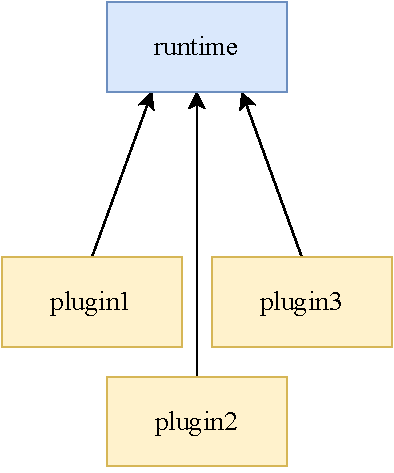
\includegraphics[width=6cm]{./Imagenes/separation-temporary.pdf}
    \caption{Ejemplo de uso de Tremor}%
    \label{fig:separation_temporary}
\end{figure}

\begin{figure}
    \centering
    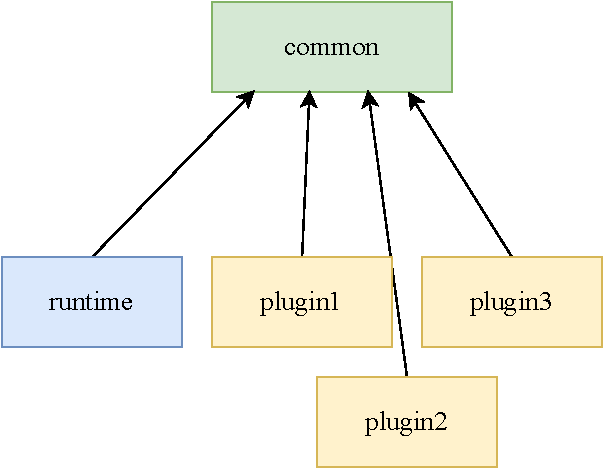
\includegraphics[width=7cm]{./Imagenes/separation.pdf}
    \caption{Ejemplo de uso de Tremor}%
    \label{fig:separation}
\end{figure}

\begin{figure}
    \centering
    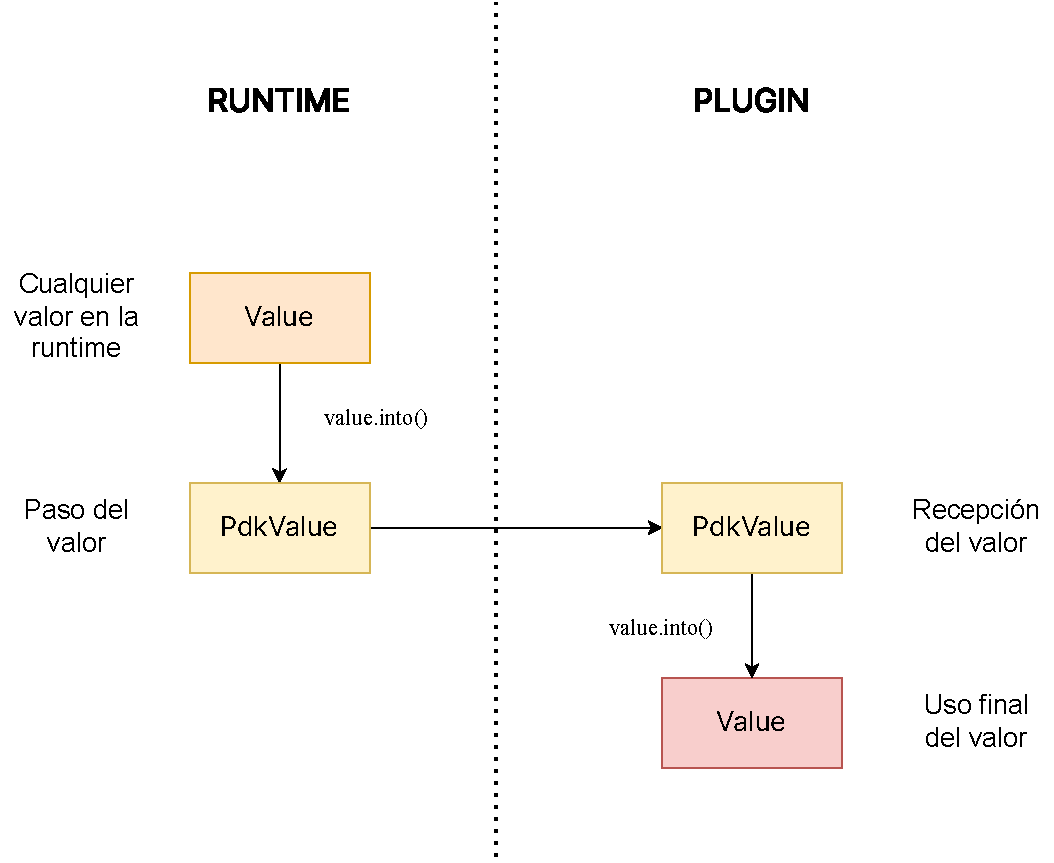
\includegraphics[width=\textwidth]{./Imagenes/simplify.pdf}
    \caption{Ejemplo de uso de Tremor}%
    \label{fig:simplify}
\end{figure}
